\documentclass[11pt]{article}

\usepackage[margin=1in]{geometry}
\usepackage[T1]{fontenc}
\usepackage{amsmath,amssymb,amsthm,mathtools}
\usepackage{enumitem}
\usepackage{booktabs}
\usepackage{microtype}
\usepackage{tikz}
\usepackage{hyperref}
\usepackage{xcolor}

\hypersetup{
  colorlinks=true,
  linkcolor=blue,
  citecolor=blue,
  urlcolor=blue
}

\newtheorem{theorem}{Theorem}[section]
\newtheorem{proposition}[theorem]{Proposition}
\newtheorem{lemma}[theorem]{Lemma}
\newtheorem{corollary}[theorem]{Corollary}
\newtheorem{definition}[theorem]{Definition}
\newtheorem{remark}[theorem]{Remark}
\newtheorem{example}[theorem]{Example}

\newcommand{\Reg}{\mathrm{Reg}}
\newcommand{\im}{\operatorname{im}}
\newcommand{\kerop}{\operatorname{ker}}
\newcommand{\supp}{\operatorname{supp}}
\newcommand{\Field}{\operatorname{Field}}
\newcommand{\Ob}{\operatorname{Ob}}
\newcommand{\dd}{\mathrm{d}}
\newcommand{\Q}{\mathbb{Q}}
\newcommand{\R}{\mathbb{R}}
\newcommand{\kfield}{\mathbb{k}}
\newcommand{\Cech}{\check{C}}
\newcommand{\CechH}{\check{H}}

\title{Associator Fields and Local-to-Global Failure\\ in Finite Compositional Structures}
\author{Duston Moore\\Independent researcher\\Edmonton, Alberta, Canada\\\texttt{dhwcmoore@gmail.com}}
\date{}

\begin{document}
\maketitle

\begin{abstract}
Compositional structure may fail at precisely the point where its local checks appear to have succeeded. This paper studies a finite categorical-algebraic setting in which local multiplication is associative on each region and pairwise overlaps carry explicit boundary corrections, but ternary composition can still depend on parenthesisation. The resulting defect is recorded as an associator field: a family of boundary-supported residues indexed by the non-empty triple overlaps of a finite regional cover. The first main result proves a localisation theorem: under support-refining boundary corrections, the associator defect of a corrected triple product is supported on the corresponding triple overlap. The second contribution separates three questions that are often conflated. Detection asks whether a defect is present, repair asks whether it can be removed by admissible changes of pairwise boundary data, and obstruction asks whether a non-removable class remains after all such repairs. Cohomology is therefore not assumed at the outset; it enters only after additional coefficient, alternation, and coherence hypotheses make the defect field into finite \v{C}ech data. The paper then gives an exact finite certificate of genuine obstruction. In a four-region seam cycle over \(\Q\), the residue \(r=(1,1,1,-2)\) is a cocycle but not a coboundary, hence determines a non-zero class in \(H^1\). The obstruction is certified both by an explicit linear contradiction and by a non-zero cycle pairing.
\end{abstract}

\noindent\textbf{Keywords:} associator; coherence; finite cohomology; local-to-global obstruction; compositional structure; categorical methods.

\medskip

\noindent\textbf{MSC 2020:} 18M05; 18A25; 18G35; 55N31; 68Q60.



\section{Introduction}

A compositional structure can pass its local tests and still fail to compose. This paper isolates one finite mechanism by which that failure occurs. The setting is deliberately elementary: a finite regional cover, supported local algebras, and boundary corrections on pairwise overlaps. Inside each region, multiplication is associative. Along each pairwise overlap, an explicit correction term records how products are reconciled across the seam. The remaining question is not unary and not binary. It is whether the two histories of ternary composition agree:
\[
a \star (b \star c)=(a \star b)\star c .
\]
The answer need not be yes. The difference
\[
a \star (b \star c)-(a \star b)\star c
\]
may be supported exactly where three regions meet. Such a defect is not an internal failure of one algebra. It is a coherence failure produced by boundary-corrected gluing.

The primitive object studied here is the \emph{associator field}. For a finite cover \(\mathcal U=(U_i)_{i\in I}\), it is a family
\[
(i,j,k)\longmapsto \alpha_{ijk}
\]
indexed by the non-empty triple overlaps of the nerve. The value \(\alpha_{ijk}\) records the parenthesisation defect associated with the triple \((U_i,U_j,U_k)\). Under the support hypotheses stated below, \(\alpha_{ijk}\) is supported on \(U_i\wedge U_j\wedge U_k\). The point is not merely that a defect can be detected. The point is that a finite compositional structure contains a level of coherence between pairwise compatibility and global gluing: every local algebra may be associative, every pairwise seam may be corrected, and yet ternary composition may still retain a residue.

This formulation places the paper in the categorical tradition of coherence and associativity, but with an important reversal of emphasis. In a monoidal category or bicategory, associators are supplied as part of the structure and then constrained by coherence axioms. Here the associator is not supplied. It is produced by the attempt to compose regional data through corrected boundaries. The question is therefore diagnostic rather than axiomatic: given finite gluing data, what associator field is generated, can it be removed by admissible boundary changes, and when does a non-removable obstruction remain?

The finite example driving the paper is a four-region seam cycle with residue
\[
r=(1,1,1,-2)\in\Q^4 .
\]
The residue is closed but not exact. It is therefore not merely a detected defect; it is not removable by the declared local bookkeeping, and it represents a non-zero class in \(H^1\). The abstract machinery is designed to explain why this is the right finite object to examine. Associator fields detect ternary failure on triple seams; admissible pairwise repair is formulated as a constrained linear problem; and the residue left by that repair problem can, under explicit hypotheses, be classified by exact rational cohomology. Section~\ref{sec:actual-witness} proves the witness twice, by an explicit linear contradiction and by a non-zero cycle pairing. Section~\ref{sec:invariance-refinement} records the declared presentation changes and refinement witnesses, and Section~\ref{sec:admissible-refinement} gives the general admissible-refinement theorem that explains their persistence.

The guiding distinction is simple. A non-zero associator value is evidence of failure, but it is not yet an obstruction. It becomes an obstruction only relative to a declared repair regime. This is why the paper keeps detection, repair, and obstruction separate. Detection is a support-local question. Repair is a question about admissible boundary gauge. Obstruction is the residue that remains after repair has failed.
\subsection{Contributions}
\label{sec:contributions}

The paper makes four contributions.

\begin{enumerate}[label=(\arabic*)]
\item \textbf{Finite associator fields.} It introduces associator fields for finite supported regional algebras. These fields record ternary coherence failure generated by boundary-corrected gluing, without assuming in advance that the defect is a cocycle or that it belongs to a pre-existing cohomology group.

\item \textbf{Localisation on triple overlaps.} In a supported regional algebra with support-refining boundary corrections, the associator defect of a corrected triple product is supported on the corresponding triple overlap (Theorem~\ref{thm:triple-localisation}). For a finite cover and a family of local inputs, the localised defects assemble into a finite field indexed by the non-empty triple overlaps of the nerve.

\item \textbf{Repair before obstruction.} Detection, repair, and obstruction are kept distinct. A non-zero associator field may be removable by admissible changes of pairwise boundary bookkeeping. It becomes obstruction-like only when its class in the repair quotient is non-zero. The repair calculus is grounded in square-zero regional extensions (Theorem~\ref{thm:square-zero-regime}), so the linearity of the repair operator is a consequence of the multiplication rule rather than an unsupported assumption.

\item \textbf{Exact finite obstruction certificate.} The four-region seam residue \(r=(1,1,1,-2)\) over \(\Q\) is a cocycle but not a coboundary, so it represents a non-zero \(H^1\) class (Proposition~\ref{prop:nonremovable}). The verdict carries two independent certificates, an inconsistent linear system and a non-zero cycle pairing, is invariant under five declared presentation changes, and persists under the declared admissible refinements.
\end{enumerate}

The order is intentional. The associator field comes first. Cohomological classification enters only after the field has been constructed, localised, and placed under a declared repair regime. The finite witness then shows how one such classification can be made exact and reproducible.
\subsection{Scope of the paper}

This paper does not give a general theory of descent, does not classify all gluing failures, does not prove full presentation invariance through arbitrary common refinement, and does not claim that every associator field is cohomological. Its scope is narrower and more exact. It isolates a finite support-refined setting in which associator defects can be produced, localised, repaired, and, in one declared finite case, certified as non-removable. The paper proves a universal admissible-refinement persistence theorem for refinements satisfying four algebraic conditions, and shows that the displayed refinement witnesses are instances of this theorem. The executable classifier accompanying the paper is exactly checked over \(\Q\) and regression tested, but it is not itself a proof-assistant verified kernel. Section~\ref{sec:scope-future} records such verification as future work.

\subsection{Running example and reader's guide}

A single informal example recurs before being computed in Section~\ref{sec:first-order}. Suppose several components maintain overlapping views of a shared structured state. Their overlaps record shared interfaces, and pairwise boundary corrections record admissible reconciliations at those interfaces. The central question is not whether each component can update its own data associatively, nor only whether every pair of components can reconcile. The question is whether threefold reconciliation is independent of parenthesisation. This running example should not be confused with the general definition. It is an interpretive aid, not a premise of the theory. The formal theory works with finite distributive lattices, supported algebras, and bilinear boundary corrections; the component model merely explains why the definitions have the shape they do.

Section~\ref{sec:related} positions the construction against coherence theory, descent, sheaf and cosheaf methods, and computational cohomology. Sections~\ref{sec:regions} and~\ref{sec:corrections} build the finite setting and prove the localisation theorem. Section~\ref{sec:dro} separates detection, repair, and obstruction, and Section~\ref{sec:first-order} gives the linearised repair calculus and grounds it in square-zero regional extensions. Section~\ref{sec:certificates} supplies the bridge from triple-seam fields to seam-cycle residues and states the finite classifier. Sections~\ref{sec:actual-witness} and~\ref{sec:invariance-refinement} prove the witness and its declared stability. Section~\ref{sec:admissible-refinement} proves the admissible-refinement persistence theorems that subsume the refinement witnesses. Section~\ref{sec:repro} makes the computational artefact reproducible, and Section~\ref{sec:scope-future} states the scope of the results and the open problems. Appendix~\ref{app:spectral} records a spectral diagnostic layer independent of the main line of argument.

\section{Related work}
\label{sec:related}

The construction of this paper sits between categorical coherence theory, descent, finite sheaf methods, and exact computational cohomology. These literatures supply much of the vocabulary, but none of them quite states the finite diagnostic problem treated here. The paper asks what defect is generated when locally associative regional products are composed through corrected pairwise seams, and when such a defect is removable by admissible boundary change.

\subsection{Coherence and associativity}

Mac Lane's coherence theorem shows that once associativity constraints in a monoidal category are supplied as natural isomorphisms satisfying the pentagon identity, all diagrams built from them commute \cite{MacLane1963,MacLane1998}. B\'enabou's bicategories generalise the pattern to weakly associative composition, again with the associator given as structure \cite{Benabou1967}. In both settings the associator is part of the definition: coherence theory asks whether supplied associators interact consistently, and answers affirmatively under the stated axioms. The present paper studies a different problem. It asks how associator defects arise when multiplication is glued from regional data with pairwise boundary corrections. The defect \(\alpha_{U,V,W}(a,b,c)\) of Section~\ref{sec:corrections} is not a supplied isomorphism and satisfies no coherence axiom by fiat; it is computed from the gluing data, may be non-zero, and may or may not be removable. In slogan form, coherence theory assumes associativity constraints as part of the structure, while this paper studies associator defects produced by boundary-corrected gluing. The two are complementary: a coherence-theoretic treatment would become available precisely when the defects studied here are shown to satisfy the relevant higher identities, which is one of the hypotheses isolated in Section~\ref{sec:certificates}.

\subsection{Descent and local-to-global obstruction}

Classical descent theory asks whether local objects together with compatibility isomorphisms on overlaps, satisfying a cocycle condition on triple overlaps, determine a global object, and it measures the failure of effective descent cohomologically \cite{Giraud1971,Vistoli2005,Weibel1994}. The local-to-global pattern of the present paper visibly resembles descent, and the triple overlap plays the same distinguished role. The difference lies in what the compatibility datum is. In descent, the datum on a pairwise overlap is an isomorphism between pullbacks, and the question is whether the given data glue. Here the datum on a pairwise overlap is a boundary-corrected multiplication, and the first object of study is not a descent datum but the associator residue produced when corrected binary gluing is iterated. Descent asks whether compatible local data determine a global object; this paper studies the residue produced when corrected binary gluing is iterated, before any global object is proposed. The repair problem of Section~\ref{sec:dro} then plays a role analogous to the freedom of modifying descent data by coboundaries, but with the admissible modifications constrained to pairwise seams by the gauge condition rather than given by a standard cochain group.

\subsection{Sheaf, cosheaf, and cellular methods}

Sheaf theory formalises exact local-to-global gluing: sections that agree on overlaps glue uniquely, and cohomology measures the failure of global sections to exist \cite{KashiwaraSchapira1990,BottTu1982}. Cellular sheaves and cosheaves transport this machinery to finite combinatorial bases, where covers, nerves, and finite cochain complexes make everything computable \cite{Curry2014,Ghrist2014,Robinson2014}. The present paper borrows the indexing discipline of this literature, in particular the nerve of a finite cover, but it deliberately does not assume the gluing axioms. The associator field is not assumed to be a sheaf cocycle. It becomes cohomological only after extra coefficient, alternation, and coherence hypotheses have been supplied, and Section~\ref{sec:certificates} states those hypotheses as explicit conditions rather than background assumptions. Cohomology is used throughout as a classification layer applied to the field, not as the primitive datum. The paper therefore occupies an intermediate level: more structured than an informal interface-failure analogy, but below the full generality of sheaf theory, descent, or factorisation algebras \cite{CostelloGwilliam2017}, whose exactness or coherence axioms are precisely what the associator field is designed to interrogate.

\subsection{Computational cohomology and certificates}

The finite classifier of Section~\ref{sec:certificates} belongs to the tradition of exact computational topology, in which finite complexes, integer or rational coboundary matrices, and exact linear algebra decide homological questions with no floating-point ambiguity \cite{EdelsbrunnerHarer2010,KaczynskiMischaikowMrozek2004,Zomorodian2005}. The specific emphasis here is on certificates. Deciding that a residue is not a coboundary by reporting that a linear solve failed requires trusting the solver. Exhibiting an explicit cycle whose pairing with the residue is non-zero requires trusting only a four-term rational calculation. The cycle-pairing lemma of Section~\ref{sec:certificates} packages that observation, and the witness of Section~\ref{sec:actual-witness} carries both certificates. The refinement witnesses of Section~\ref{sec:invariance-refinement} are certificates in the same sense: each is a self-contained cycle-pairing verification in the refined complex.

\subsection{Verified certificate checking}

A certificate is only as trustworthy as its checker. The programme of proof-carrying code and certified computation replaces trust in a large tool by trust in a small verified checker \cite{Necula1997}, and proof assistants such as Rocq make it possible to prove the checker itself sound \cite{Rocq2025}. The classifier accompanying this paper is tested Python with property-based regression against the cycle-pairing criterion; it is not a verified kernel. Section~\ref{sec:scope-future} states the minimal soundness theorem that a verified version would establish, namely that the verdict \texttt{nontrivial\_H1\_obstruction} implies a genuine non-zero \(H^1\) class. The mathematics of this paper does not depend on that step, because the displayed witness is proved by hand, but the step is the natural continuation of the certificate discipline adopted here.

\subsection{Position of the contribution}

The contribution is not a new proof of descent, not a replacement for \v{C}ech cohomology, and not a general theory of weak higher categories. It is a finite categorical-algebraic mechanism for producing, localising, and testing associator defects generated by boundary-corrected gluing. The novelty is the separation between the associator field as a primitive defect datum and its later classification by repair quotients or cohomology. This separation matters because it prevents a detected defect from being treated prematurely as an obstruction. Only after the admissible repair directions have been fixed can a residual class be called non-removable. The four-region witness gives a fully explicit finite case in which that process terminates in a certified obstruction.

\section{Finite regional covers and supported algebras}
\label{sec:regions}

\begin{definition}[Region system]
A region system is a finite distributive lattice
\[
(\Reg,\leq,\bot,\top,\vee,\wedge).
\]
The elements of \(\Reg\) are called regions. The join \(\vee\) is read as regional union, and the meet \(\wedge\) as overlap. No underlying point-set representation is assumed.
\end{definition}

\begin{remark}[Terminology]
The term region system is used only as a neutral name for a finite distributive lattice whose elements index supports and overlaps. No new foundational claim is attached to the terminology. Readers who prefer standard vocabulary may read every occurrence as a finite distributive lattice, with covers and nerves defined below exactly as for finite covers in combinatorial topology. The lattice-theoretic formulation is chosen because the constructions use only joins, meets, and the order, so that a point-set realisation, while available in examples, is never required by a proof.
\end{remark}

\begin{definition}[Finite cover]
Let \(R\in \Reg\). A finite family \(\mathcal U=(U_i)_{i\in I}\) is a cover of \(R\) if
\[
R=\bigvee_{i\in I}U_i.
\]
For every non-empty finite subset \(J\subseteq I\), write
\[
U_J=\bigwedge_{j\in J}U_j.
\]
For \(J=\{i_0,\ldots,i_n\}\), we also write \(U_{i_0\cdots i_n}\).
\end{definition}

\begin{definition}[Nerve]
The nerve \(N(\mathcal U)\) is the finite simplicial complex whose \(n\)-simplices are the non-empty subsets \(J\subseteq I\) with \(|J|=n+1\) and
\[
U_J\neq \bot.
\]
Thus vertices are regions, edges are non-empty pairwise overlaps, and triangles are non-empty triple overlaps.
\end{definition}

\begin{remark}[Why the nerve is not yet the answer]
The nerve records the incidence pattern of overlaps. It does not by itself say what lives on those overlaps. The associator field constructed below uses the nerve as an index shape, but its values come from the regional algebra and its boundary corrections.
\end{remark}

\begin{definition}[Ordered simplices]
When an ordered tuple \((i_0,\ldots,i_n)\) is used, its entries are assumed to be pairwise distinct unless explicitly stated otherwise. Such a tuple represents an oriented simplex of the nerve whenever \(U_{i_0\cdots i_n}\neq \bot\).
\end{definition}

The localisation theorem needs a disciplined notion of support. The next definition supplies it. The algebras are not required to be unital, since extension by zero is one intended model.

\begin{definition}[Supported regional algebra]
\label{def:supported-algebra}
Let \(k\) be a commutative ring. A supported regional algebra on \(\Reg\) consists of the following data.

\begin{enumerate}[label=(\roman*)]
\item For each region \(R\in \Reg\), a not-necessarily-unital associative \(k\)-algebra \(A(R)\).

\item For each inclusion \(R\leq S\), an injective \(k\)-algebra homomorphism
\[
\iota_{RS}:A(R)\to A(S),
\]
not required to preserve units, satisfying
\[
\iota_{RR}=\mathrm{id},
\qquad
\iota_{ST}\circ \iota_{RS}=\iota_{RT}
\quad (R\leq S\leq T).
\]

\item An intersection support-refinement rule: if \(x\in A(S)\) is supported on \(R\leq S\), and \(y\in A(S)\) is supported on \(T\leq S\), then \(xy\) is supported on \(R\wedge T\).
\end{enumerate}

Here an element \(x\in A(S)\) is supported on \(R\leq S\) when
\[
x\in \im(\iota_{RS}).
\]
Because \(\iota_{RS}\) is injective, such an element has a unique representative in \(A(R)\), denoted \(x\rvert_R\). No minimal support is assumed: an element may be supported on several regions, and \(x\rvert_R\) always refers to the representative relative to a specified supporting region \(R\), not to a smallest such region.
\end{definition}

\begin{example}[Canonical example: dual-number seam annotations]
\label{ex:canonical}
The simplest instance carries every construction of the paper. Let \(k\) be a field and let every region carry the dual-number algebra
\[
A(R)=D=k[\varepsilon]/(\varepsilon^2),
\]
with all extension maps the identity, so that every element is supported on every region. The primary channel, the coefficient of \(1\), carries an ordinary value such as an interval width; the boundary channel, the coefficient of \(\varepsilon\), carries a square-zero seam annotation such as a reconciliation cost. Products of two annotations vanish because \(\varepsilon^2=0\). This scalar model suppresses the proof-carrying support representatives of the general theory, but it exhibits the boundary corrections, the first-order regime, and the associator defect in fully computable form, and it is the model computed in Section~\ref{sec:first-order}. Extension by zero on a genuine lattice of regions supplies a second model in which the support structure is non-trivial.
\end{example}

\begin{remark}[Extension is not restriction]
The maps \(\iota_{RS}\) go from smaller regions to larger regions. They are extension maps. The notation \(x\rvert_R\) is used only when \(x\) is already known to lie in the image of \(\iota_{RS}\). It is not a general restriction map \(A(S)\to A(R)\).
\end{remark}

\begin{lemma}[Supported multiplication representative]
\label{lem:supported-mult}
Let \(R,T\leq S\). If \(x\in A(S)\) is supported on \(R\), and \(y\in A(S)\) is supported on \(T\), then \(xy\) has a unique representative
\[
(xy)\rvert_{R\wedge T}\in A(R\wedge T).
\]
\end{lemma}

\begin{proof}
By the support-refinement rule, \(xy\) is supported on \(R\wedge T\). Hence \(xy\in \im(\iota_{R\wedge T,S})\). Since \(\iota_{R\wedge T,S}\) is injective, the representative is unique.
\end{proof}

\section{Boundary corrections and associator fields}
\label{sec:corrections}

A boundary correction records a contribution assigned to the seam where two regions are glued.

\begin{definition}[Boundary correction]
A boundary correction on a supported regional algebra is a family of \(k\)-bilinear maps
\[
\beta_{U,V}:A(U)\otimes_k A(V)\to A(U\wedge V)
\]
for ordered pairs of regions \((U,V)\).
\end{definition}

\begin{definition}[Support-refining boundary correction]
A boundary correction \(\beta\) is support-refining if the following holds. Let \(X\leq U\) and \(Y\leq V\). If \(a\in A(U)\) is supported on \(X\) and \(b\in A(V)\) is supported on \(Y\), then the value \(\beta_{U,V}(a,b)\in A(U\wedge V)\) is supported on
\[
X\wedge Y\leq U\wedge V.
\]
\end{definition}

\begin{remark}[Running example]
In the canonical model of Example~\ref{ex:canonical}, a boundary correction can be as simple as an on-off seam annotation,
\[
\beta_{X,Y}(a,b)=\chi(X,Y)\pi(a)\pi(b)\varepsilon,
\]
where \(\pi\) projects onto the primary channel and \(\chi(X,Y)=1\) when two interval views properly partially overlap and \(\chi(X,Y)=0\) otherwise. The general definition allows more than this scalar toy model, but the toy model explains why \(\beta\) is bilinear and why its value belongs to the overlap algebra.
\end{remark}

\begin{definition}[Raw overlap product]
For \(a\in A(U)\) and \(b\in A(V)\), set \(S=U\vee V\). Extend both elements to \(S\), multiply there, and take the supported representative on \(U\wedge V\):
\[
m_{U,V}(a,b):=\bigl(\iota_{US}(a)\iota_{VS}(b)\bigr)\rvert_{U\wedge V}\in A(U\wedge V).
\]
This is well-defined by Lemma~\ref{lem:supported-mult}.
\end{definition}

\begin{definition}[Boundary-corrected product]
For \(a\in A(U)\) and \(b\in A(V)\), define
\[
a\star_{U,V} b
:=
\iota_{U\wedge V,U\vee V}\bigl(m_{U,V}(a,b)+\beta_{U,V}(a,b)\bigr)
\in A(U\vee V).
\]
\end{definition}

\begin{remark}[Boundary interaction product]
The product \(\star_{U,V}\) is a boundary interaction product. Its value lies in the ambient algebra \(A(U\vee V)\), but its support is contained in \(U\wedge V\). This is intentional. The paper isolates the seam contribution rather than modelling arbitrary independent interior multiplication on \(U\vee V\).
\end{remark}

\begin{lemma}[Support of the corrected product]
\label{lem:corrected-support}
For \(a\in A(U)\) and \(b\in A(V)\), the element
\[
a\star_{U,V}b\in A(U\vee V)
\]
is supported on \(U\wedge V\).
\end{lemma}

\begin{proof}
Both \(m_{U,V}(a,b)\) and \(\beta_{U,V}(a,b)\) lie in \(A(U\wedge V)\). The corrected product is obtained by applying \(\iota_{U\wedge V,U\vee V}\) to their sum.
\end{proof}

\subsection{The associator defect}

Let \(U,V,W\in \Reg\), and let
\[
a\in A(U),\qquad b\in A(V),\qquad c\in A(W).
\]
There are two corrected ways to multiply these three elements:
\[
(a\star_{U,V}b)\star_{U\vee V,W}c,
\qquad
 a\star_{U,V\vee W}(b\star_{V,W}c).
\]
Both lie in \(A(U\vee V\vee W)\). Figure~\ref{fig:triple} shows the configuration.

\begin{figure}[t]
\centering
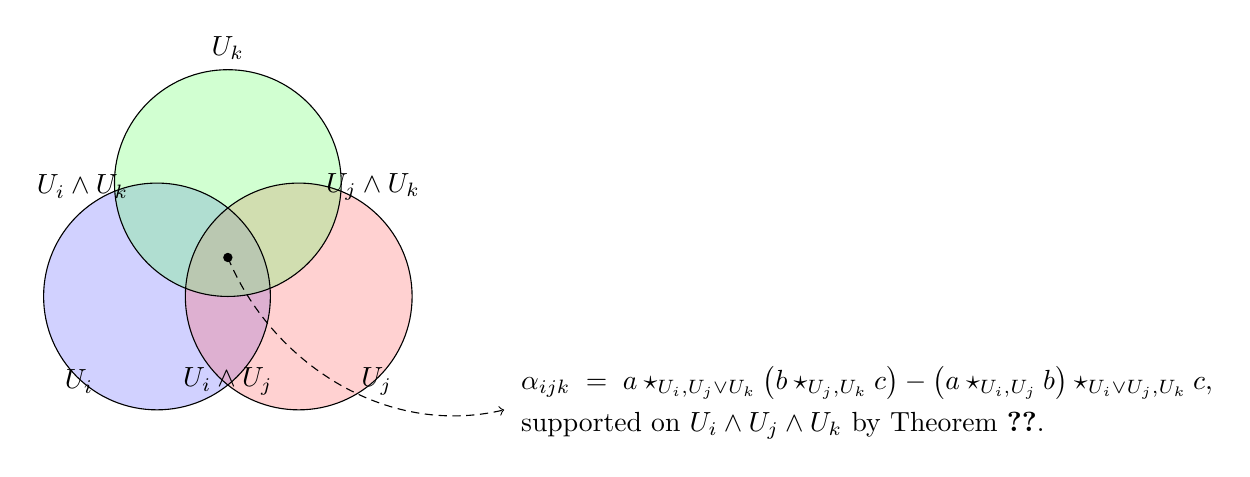
\begin{tikzpicture}[scale=0.9]
\begin{scope}[opacity=0.30]
\fill[blue!60]  (0,0) circle (1.6);
\fill[red!60]   (2.0,0) circle (1.6);
\fill[green!60] (1.0,1.6) circle (1.6);
\end{scope}
\draw (0,0) circle (1.6);
\draw (2.0,0) circle (1.6);
\draw (1.0,1.6) circle (1.6);
\node at (-1.1,-1.2) {$U_i$};
\node at (3.1,-1.2) {$U_j$};
\node at (1.0,3.5) {$U_k$};
\node at (1.0,-1.2) {$U_i\wedge U_j$};
\node at (-1.05,1.55) {$U_i\wedge U_k$};
\node at (3.05,1.55) {$U_j\wedge U_k$};
\node at (1.0,0.55) [circle,fill=black,inner sep=1.2pt] {};
\draw[->,densely dashed,thin] (1.0,0.55) .. controls (1.6,-0.9) and (3.2,-2.0) .. (4.9,-1.6);
\node[align=left,right] at (5.0,-1.5)
  {$\alpha_{ijk}
    \;=\;
    a\star_{U_i,U_j\vee U_k}\bigl(b\star_{U_j,U_k}c\bigr)
    -\bigl(a\star_{U_i,U_j}b\bigr)\star_{U_i\vee U_j,U_k}c,$\\[3pt]
   supported on $U_i\wedge U_j\wedge U_k$ by Theorem~\ref{thm:triple-localisation}.};
\end{tikzpicture}
\caption{Three regions, their pairwise overlaps, and the triple overlap. The two parenthesised histories of corrected composition are compared; Theorem~\ref{thm:triple-localisation} forces their difference, the associator defect \(\alpha_{ijk}\), onto the triple overlap.}
\label{fig:triple}
\end{figure}

\begin{definition}[Associator defect]
The associator defect of \(a,b,c\) over \((U,V,W)\) is
\[
\alpha_{U,V,W}(a,b,c)
:=
 a\star_{U,V\vee W}(b\star_{V,W}c)
-
 (a\star_{U,V}b)\star_{U\vee V,W}c
\in A(U\vee V\vee W).
\]
This is the right-minus-left convention used throughout the paper.
\end{definition}

\begin{lemma}[Extension preserves support]
\label{lem:extension-support}
Let \(R\leq T\leq S\). If \(x\in A(T)\) is supported on \(R\), then \(\iota_{TS}(x)\in A(S)\) is supported on \(R\).
\end{lemma}

\begin{proof}
Since \(x\) is supported on \(R\), there is \(x_R\in A(R)\) such that \(x=\iota_{RT}(x_R)\). Hence
\[
\iota_{TS}(x)=\iota_{TS}\iota_{RT}(x_R)=\iota_{RS}(x_R),
\]
so \(\iota_{TS}(x)\in \im(\iota_{RS})\).
\end{proof}

\begin{theorem}[Triple-overlap localisation]\label{thm:triple-localisation}
Assume that \(\beta\) is support-refining. Then
\[
\alpha_{U,V,W}(a,b,c)
\]
is supported on
\[
U\wedge V\wedge W.
\]
Equivalently, there is a unique element
\[
\widetilde\alpha_{U,V,W}(a,b,c)\in A(U\wedge V\wedge W)
\]
such that
\[
\iota_{U\wedge V\wedge W,U\vee V\vee W}\bigl(\widetilde\alpha_{U,V,W}(a,b,c)\bigr)
=
\alpha_{U,V,W}(a,b,c).
\]
\end{theorem}

\begin{proof}
Set \(S=U\vee V\vee W\). Consider first the left-parenthesised product
\[
(a\star_{U,V}b)\star_{U\vee V,W}c.
\]
By Lemma~\ref{lem:corrected-support}, the inner product \(a\star_{U,V}b\) is supported on \(U\wedge V\) inside \(A(U\vee V)\). By Lemma~\ref{lem:extension-support}, after extension to \(S\) it remains supported on \(U\wedge V\). The element \(c\), extended from \(W\) to \(S\), is supported on \(W\). By the intersection support-refinement rule, the raw outer product of these two elements is supported on
\[
(U\wedge V)\wedge W=U\wedge V\wedge W.
\]
The outer correction \(\beta_{U\vee V,W}(a\star_{U,V}b,c)\) is supported on \((U\wedge V)\wedge W=U\wedge V\wedge W\) as well, by support refinement for \(\beta\) applied to the first argument supported on \(U\wedge V\) and the second supported on \(W\). Hence the left-parenthesised product is supported on \(U\wedge V\wedge W\).

The right-parenthesised product
\[
a\star_{U,V\vee W}(b\star_{V,W}c)
\]
is treated by the same argument with the roles of the union terms exchanged. By Lemma~\ref{lem:corrected-support}, the inner product \(b\star_{V,W}c\) is supported on \(V\wedge W\), and by Lemma~\ref{lem:extension-support} it remains so after extension to \(S\). The element \(a\) is supported on \(U\). The raw outer product is therefore supported on \(U\wedge (V\wedge W)\), and the outer correction \(\beta_{U,V\vee W}(a,b\star_{V,W}c)\) is supported on the same overlap by support refinement. Since the meet is associative,
\[
U\wedge (V\wedge W)=U\wedge V\wedge W,
\]
so the right-parenthesised product is supported on \(U\wedge V\wedge W\) as well.

Both parenthesised products are therefore supported on \(U\wedge V\wedge W\), and so is their difference. The uniqueness of the representative \(\widetilde\alpha_{U,V,W}(a,b,c)\) follows from injectivity of the extension map \(\iota_{U\wedge V\wedge W,S}\).
\end{proof}

\begin{remark}[Localisation, not mere failure]
Theorem~\ref{thm:triple-localisation} says more than that associativity can fail. It says that, under explicit support discipline, the failure is forced onto the common seam of the three regions. The defect is locally supported but globally induced.
\end{remark}

\subsection{Associator fields}

We now pass from one triple to a finite cover.

\begin{definition}[Input family]
Let \(\mathcal U=(U_i)_{i\in I}\) be a finite cover. An input family on \(\mathcal U\) is a choice
\[
a=(a_i)_{i\in I},
\qquad
 a_i\in A(U_i).
\]
\end{definition}

\begin{definition}[Associator field]
Let \(\mathcal U=(U_i)_{i\in I}\) be a finite cover and let \(a=(a_i)_{i\in I}\) be an input family. The associator field of \(a\) is the assignment
\[
\mathcal A_a:(i,j,k)\longmapsto
\widetilde\alpha_{U_i,U_j,U_k}(a_i,a_j,a_k)
\in A(U_i\wedge U_j\wedge U_k)
\]
for ordered triples of pairwise distinct indices with \(U_i\wedge U_j\wedge U_k\neq \bot\).
\end{definition}

\begin{remark}[The field is ordered, not alternating]
No antisymmetry in \((i,j,k)\) is assumed. The field is ordered because the corrected product need not be symmetric in its inputs, so in general
\[
\mathcal A_a(i,j,k)\neq -\mathcal A_a(j,i,k).
\]
This matters later: passing to a \v{C}ech cochain requires an explicit alternation hypothesis, rather than following automatically.
\end{remark}

\begin{remark}[Field before class]
The associator field is the primitive datum of this paper. Cohomology is one possible classification of that datum under additional hypotheses, supplied in Section~\ref{sec:certificates}. The field is not automatically a cocycle, a cohomology class, or a harmonic form; it is the finite record produced by gluing, and further structures may classify it without constituting it.
\end{remark}

The field has three primitive features. Incidence: it is defined only where the triple overlap exists. Support: each value lives on the corresponding triple overlap. History: each value compares two parenthesised histories of composition. This gives the first conceptual separation,
\[
\text{interior validity}\neq \text{pairwise compatibility}\neq \text{triple coherence}.
\]
Interior validity means that each \(A(U_i)\) is associative. Pairwise compatibility means that each seam \(U_i\wedge U_j\) carries a specified correction. Triple coherence means that the corrections do not leave an associator residue on \(U_i\wedge U_j\wedge U_k\).

\section{Detection, repair, and obstruction}
\label{sec:dro}

The associator field invites three different questions. They should be kept separate, and the separation is the organising frame of the rest of the paper.

\subsection{Detection}

Detection asks whether and where the field is non-zero:
\[
\mathcal A_a(i,j,k)\neq 0.
\]
This is the most primitive diagnostic. It identifies triple seams at which pairwise-corrected composition still depends on parenthesisation.

\subsection{Repair}

Repair asks whether the defect can be removed by changing pairwise boundary bookkeeping.

\begin{definition}[Boundary gauge, informal finite version]
A boundary gauge is an admissible change
\[
\beta_{U,V}\longmapsto \beta_{U,V}+\Theta_{U,V},
\]
where each
\[
\Theta_{U,V}:A(U)\otimes_k A(V)\to A(U\wedge V)
\]
is bilinear and support-refining.
\end{definition}

\begin{definition}[Admissible gauge in the first-order regime]
In the first-order boundary regime of Section~\ref{sec:first-order}, a gauge \(\Theta\) is admissible if each \(\Theta_{U,V}\) is bilinear and support-refining, its outputs lie in the relevant boundary ideal after extension to the ambient region, and it vanishes whenever either argument lies in the relevant boundary ideal. The informal use of admissibility above is made precise by this condition once the first-order regime has been fixed.
\end{definition}

The word admissible is doing real work. A repair is not an arbitrary assignment to triple overlaps. It must be induced by changes at pairwise seams. Thus repair is a constrained problem: can pairwise changes cancel a triple-seam field?

In a linearised or first-order regime, boundary gauges determine a variation map
\[
D:G^1\to \Field^2,
\]
from admissible pairwise gauges to associator fields. Here \(G^1\) denotes the \(k\)-module of admissible pairwise gauge families \((\Theta_{ij})\), and \(\Field^2\) denotes the \(k\)-module of triple-indexed assignments
\[
F_{ijk}\in A(U_i\wedge U_j\wedge U_k),
\]
both for the fixed cover and input family under discussion. A field \(\mathcal A\) is repairable when
\[
\mathcal A\in \im D.
\]

\begin{definition}[Repair quotient]
In a fixed first-order regime with variation map \(D:G^1\to \Field^2\), define the repair quotient
\[
\Ob_D:=\Field^2/\im D.
\]
The class of \(\mathcal A\) in \(\Ob_D\) records the part of the associator field that is not removed by admissible pairwise boundary gauges.
\end{definition}

\begin{remark}[Why this is not yet \v{C}ech cohomology]
The operator \(D\) need not be the ordinary \v{C}ech coboundary. It is determined by how the corrected product is parenthesised and by which boundary gauges are admissible. Ordinary \v{C}ech cohomology appears only when \(D\) can be identified with a \v{C}ech differential in a specified coefficient system, which is the subject of Section~\ref{sec:certificates}.
\end{remark}

\subsection{Obstruction}

Obstruction is the modal status of a defect after repair has been attempted. A non-zero value
\[
\mathcal A_a(i,j,k)\neq 0
\]
is not yet an obstruction. It may be removable by a change of pairwise bookkeeping. It becomes obstruction-like only when its class in the repair quotient is non-zero:
\[
[\mathcal A_a]_D\neq 0.
\]
Thus obstruction is not the first object. It is what remains when admissible repairs fail.

\section{First-order repair calculus}
\label{sec:first-order}

This section records the finite first-order shape of repair. It is a linearised repair calculus, not a universal repair theorem: it computes the variation of the associator defect under admissible gauges in a regime where second-order boundary interactions vanish, and it makes no claim outside that regime. The regime is first stated axiomatically and then answered by construction. Square-zero regional extensions, introduced in Section~\ref{sec:square-zero}, supply a natural model in which every axiom is a consequence of the multiplication rule, so the linearity of the repair operator follows from the vanishing of squared boundary terms rather than being imposed.

\subsection{The first-order axioms}

\begin{definition}[First-order boundary regime]
A boundary-corrected regional algebra is first-order if, for every region \(S\), there is a two-sided \(k\)-submodule ideal \(B(S)\subseteq A(S)\), called the boundary ideal, such that:

\begin{enumerate}[label=(\roman*)]
\item for every pair \(U,V\) and all inputs \(a,b\), the extended correction \(\iota_{U\wedge V,U\vee V}(\beta_{U,V}(a,b))\) and the extended gauge \(\iota_{U\wedge V,U\vee V}(\Theta_{U,V}(a,b))\) lie in \(B(U\vee V)\);
\item \(B(S)^2=0\);
\item multiplication by ordinary elements sends boundary elements to boundary elements;
\item extension maps preserve the boundary ideals;
\item for every pair \(U,V\), the maps \(\beta_{U,V}\) and every admissible gauge \(\Theta_{U,V}\) factor through
\[
(A(U)/B(U))\otimes_k(A(V)/B(V)),
\]
equivalently they vanish whenever either input lies in the relevant boundary ideal.
\end{enumerate}
\end{definition}

In such a regime, products of two newly inserted boundary corrections vanish. The effect of changing \(\beta\) by a gauge \(\Theta\) is therefore linear to first order.

\begin{remark}[Running example]
The dual-number model of Example~\ref{ex:canonical} is the simplest first-order regime, with boundary ideal \(k\varepsilon\). Since \(\varepsilon^2=0\), two newly inserted reconciliation annotations do not multiply into a second-order ordinary effect.
\end{remark}

\subsection{The first-order repair variation}

\begin{proposition}[First-order repair variation]
\label{prop:four-term}
Let \(A\) be a first-order boundary regime, let \(a\in A(U)\), \(b\in A(V)\), \(c\in A(W)\), write \(\Lambda=U\wedge V\wedge W\), and let \(m_{X,Y}\) denote the uncorrected raw overlap product. If the boundary correction \(\beta\) is changed by an admissible first-order gauge \(\Theta\), then the associator defect, with the right-minus-left convention, changes by \(D\Theta_{U,V,W}(a,b,c)\), the unique element of \(A(\Lambda)\) given by
\begin{align*}
D\Theta_{U,V,W}(a,b,c)
={}&
\Bigl[\Theta_{U,V\vee W}\bigl(a,\iota_{V\wedge W,V\vee W}(m_{V,W}(b,c))\bigr)\Bigr]\rvert_\Lambda \\
&+m_{U,V\wedge W}\bigl(a,\Theta_{V,W}(b,c)\bigr) \\
&-\Bigl[\Theta_{U\vee V,W}\bigl(\iota_{U\wedge V,U\vee V}(m_{U,V}(a,b)),c\bigr)\Bigr]\rvert_\Lambda \\
&-m_{U\wedge V,W}\bigl(\Theta_{U,V}(a,b),c\bigr).
\end{align*}
\end{proposition}

\begin{proof}
Expand the two parenthesised products after replacing \(\beta\) by \(\beta+\Theta\). Because the regime is first-order, every term carrying two newly inserted boundary corrections vanishes, and the admissible gauge maps ignore arguments that are already boundary elements. Hence the variation is linear in \(\Theta\).

The right-parenthesised product contributes two first-order terms: the outer gauge evaluated on the raw inner product, after the inner product is extended from \(V\wedge W\) to \(V\vee W\), and the raw outer product evaluated on the inner gauge. The first term initially lands in a larger overlap algebra and is reduced to \(\Lambda\) by \(\rvert_\Lambda\). These are the first two displayed terms.

The left-parenthesised product contributes the corresponding two terms with negative sign, because the associator defect is right-minus-left. Every displayed map has a determined source and target. The bracketed terms require the support witnesses that identify their outputs with elements supported on \(\Lambda\). With those witnesses, support refinement places every displayed term on \(\Lambda\), and injectivity of the extension maps gives the stated representatives in \(A(\Lambda)\).
\end{proof}

\begin{remark}[The warning hidden in the formula]
The four-term expression is the native repair operator for this parenthesised gluing problem. It is not automatically the ordinary three-face \v{C}ech formula. To obtain ordinary \v{C}ech cohomology, one must impose additional identifications that replace the mixed union terms by the corresponding face restrictions in a genuine coefficient system.
\end{remark}

\subsection{A worked scalar instance}
\label{sec:interval-example}

The canonical model of Example~\ref{ex:canonical} makes the calculus concrete; Section~\ref{sec:square-zero} will embed it as the degenerate case of a genuinely regional model. Take all local algebras equal to \(D=k[\varepsilon]/(\varepsilon^2)\) with boundary ideal \(k\varepsilon\), all extension maps identities, and corrections
\[
\beta_{P,Q}(x,y)=\lambda_{P,Q}\,\pi(x)\pi(y)\,\varepsilon
\]
for constants \(\lambda_{P,Q}\in k\), where \(\pi(x_0+x_1\varepsilon)=x_0\). This is a scalar coefficient reduction of the regional theory, not a faithful model of minimal support: with identity extensions every element is supported on every region, so the calculation computes the seam coefficients while suppressing the proof-carrying support representatives of the general theory. A direct expansion gives
\[
\widetilde\alpha_{U,V,W}(a,b,c)=\Delta_{U,V,W}\,a_0b_0c_0\,\varepsilon,
\qquad
\Delta_{U,V,W}
=
\lambda_{V,W}-\lambda_{U\vee V,W}+\lambda_{U,V\vee W}-\lambda_{U,V},
\]
which is the four-term expression of Proposition~\ref{prop:four-term} in scalar form. If this expression is induced by an admissible pairwise gauge, the defect is repairable; if not, it persists in the repair quotient.

\begin{example}[Interval reconciliation]
\label{ex:interval}
Instantiate the constants by the reconciliation indicator \(\lambda_{X,Y}=\chi(X,Y)\), where \(\chi(X,Y)=1\) when the intervals \(X\) and \(Y\) properly partially overlap, meaning \(X\cap Y\neq\varnothing\) with neither contained in the other, and \(\chi(X,Y)=0\) otherwise. For three nodes with interval views \(U=[0,4]\), \(V=[2,6]\), \(W=[4,8]\), all four binary gluing sites reconcile, so
\[
\widetilde\alpha_{U,V,W}(1,1,1)=(1-1+1-1)\varepsilon=0,
\]
and both parenthesisations incur the same first-order cost. Now reposition the third node inside the combined span of the first two while it still crosses their interface: \(U=[0,4]\), \(V=[2,6]\), \(W=[1,5]\). Then \(W\subseteq U\vee V\) but \(W\) is contained in neither \(U\) nor \(V\), so \(\chi(U\vee V,W)=0\) while the other three indicators remain \(1\), and
\[
\widetilde\alpha_{U,V,W}(1,1,1)=(1-0+1-1)\varepsilon=\varepsilon\neq 0
\]
on the triple seam \(U\wedge V\wedge W=[2,4]\). The non-zero residue is produced neither by an interior failure of any local algebra nor by a degenerate overlap. It appears exactly when a region is absorbed by a union while still crossing the interface between the union's components, and it demonstrates the governing sentence of the introduction in the smallest possible model.
\end{example}

\subsection{Square-zero regional extensions}
\label{sec:square-zero}

The axioms above prompt an immediate question, and a reviewer would be right to press it: why should the repair operator be linear, and why does the variation formula of Proposition~\ref{prop:four-term} have exactly four terms with no quadratic corrections? Answering by assumption is legitimate but weak. This subsection answers by construction. The construction is the regional form of a square-zero extension: the boundary layer is an ordinary bimodule glued onto the regional algebra with a multiplication that contains no boundary-times-boundary term, so second-order seam interactions vanish identically rather than by decree.

\begin{definition}[Regional boundary bimodule]
\label{def:boundary-bimodule}
Let \(A_0\) be a supported regional algebra on \(\Reg\) in the sense of Definition~\ref{def:supported-algebra}, with extension maps \(\iota^0_{RS}\). A regional boundary bimodule for \(A_0\) assigns to each region \(S\) an \(A_0(S)\)-bimodule \(B(S)\), together with injective \(k\)-linear extension maps
\[
\iota^B_{RS}:B(R)\to B(S)
\qquad(R\leq S)
\]
satisfying \(\iota^B_{RR}=\mathrm{id}\) and \(\iota^B_{ST}\circ\iota^B_{RS}=\iota^B_{RT}\), such that the following two compatibilities hold. First, extension commutes with the actions: for \(R\leq S\), \(x\in A_0(R)\), and \(\xi\in B(R)\),
\[
\iota^B_{RS}(x\cdot\xi)=\iota^0_{RS}(x)\cdot\iota^B_{RS}(\xi),
\qquad
\iota^B_{RS}(\xi\cdot x)=\iota^B_{RS}(\xi)\cdot\iota^0_{RS}(x).
\]
Second, the actions refine support by intersection: if \(x\in A_0(S)\) is supported on \(X\leq S\) and \(\xi\in B(S)\) is supported on \(Y\leq S\), then \(x\cdot\xi\) and \(\xi\cdot x\) are supported on \(X\wedge Y\). Support in \(B\) means membership in the image of the relevant \(\iota^B\), exactly as for the algebra.
\end{definition}

\begin{definition}[Square-zero regional extension]
\label{def:square-zero}
Given \(A_0\) and a regional boundary bimodule \(B\), the square-zero regional extension \(A=A_0\ltimes B\) assigns to each region \(S\) the \(k\)-module
\[
A(S)=A_0(S)\oplus B(S)
\]
with multiplication
\[
(x,\xi)(y,\eta)=(xy,\;x\cdot\eta+\xi\cdot y)
\]
and extension maps \(\iota_{RS}=\iota^0_{RS}\oplus\iota^B_{RS}\). There is no \(\xi\eta\) term. The submodule \(B(S)\), identified with \(0\oplus B(S)\), is a two-sided ideal with \(B(S)^2=0\), called the boundary ideal, and the projection \(\pi:A(S)\to A_0(S)\) onto the first summand is an algebra homomorphism with kernel \(B(S)\).
\end{definition}

\begin{lemma}[Square-zero extensions are supported regional algebras]
\label{lem:square-zero-supported}
Let \(A=A_0\ltimes B\) be a square-zero regional extension. Then each \(A(S)\) is an associative \(k\)-algebra, each \(\iota_{RS}\) is an injective algebra homomorphism satisfying the functoriality conditions, and the intersection support-refinement rule of Definition~\ref{def:supported-algebra} holds.
\end{lemma}

\begin{proof}
Associativity is the standard square-zero calculation: both triple products of \((x,\xi)\), \((y,\eta)\), \((z,\zeta)\) equal \((xyz,\;xy\cdot\zeta+x\cdot\eta\cdot z+\xi\cdot yz)\), using associativity of \(A_0(S)\) and the bimodule axioms, since every term containing two boundary factors vanishes. Injectivity and functoriality of \(\iota_{RS}\) hold componentwise, and \(\iota_{RS}\) is an algebra homomorphism because both components of the multiplication commute with extension, the second by the first compatibility of Definition~\ref{def:boundary-bimodule}. For support refinement, an element \((x,\xi)\in A(S)\) is supported on \(R\) precisely when \(x\) and \(\xi\) are separately supported on \(R\), since \(\iota_{RS}\) acts componentwise. If \((x,\xi)\) is supported on \(R\) and \((y,\eta)\) on \(T\), then \(xy\) is supported on \(R\wedge T\) by the rule for \(A_0\), and \(x\cdot\eta\) and \(\xi\cdot y\) are supported on \(R\wedge T\) by the second compatibility of Definition~\ref{def:boundary-bimodule}. Hence the product is supported on \(R\wedge T\).
\end{proof}

\begin{definition}[Seam corrections and gauges in a square-zero extension]
\label{def:seam-correction}
A seam correction datum on \(A=A_0\ltimes B\) is a family of \(k\)-bilinear, support-refining maps
\[
\lambda_{U,V}:A_0(U)\otimes_k A_0(V)\to B(U\wedge V)
\]
for ordered pairs of regions. It induces the boundary correction
\[
\beta_{U,V}(a,b):=\bigl(0,\;\lambda_{U,V}(\pi a,\pi b)\bigr)\in A(U\wedge V),
\]
so that the correction is computed from ordinary data only and its value lies entirely in the boundary component. Admissible gauges are defined by the same construction: a gauge datum is a second family \(\nu_{U,V}\) of the same type, inducing \(\Theta_{U,V}(a,b)=(0,\nu_{U,V}(\pi a,\pi b))\).
\end{definition}

\begin{theorem}[Square-zero extensions are first-order boundary regimes]
\label{thm:square-zero-regime}
Let \(A=A_0\ltimes B\) be a square-zero regional extension, let \(\beta\) be induced by a seam correction datum, and let the admissible gauges be those induced by gauge data. Then \(A\), with the boundary ideals \(B(S)\), satisfies all five axioms of the first-order boundary regime. Consequently the variation formula of Proposition~\ref{prop:four-term} holds in \(A\), with the linearity of the repair operator following from \(B(S)^2=0\) rather than by hypothesis.
\end{theorem}

\begin{proof}
Each axiom is verified directly from the construction. For the first, the values of \(\beta_{U,V}\) and of every admissible \(\Theta_{U,V}\) lie in \(0\oplus B(U\wedge V)\) by Definition~\ref{def:seam-correction}, and extension maps act componentwise, so the extended values lie in \(B(U\vee V)\). For the second, the multiplication of Definition~\ref{def:square-zero} contains no boundary-times-boundary term, so \(B(S)^2=0\) identically. For the third, \((x,\xi)(0,\eta)=(0,x\cdot\eta)\) and \((0,\eta)(x,\xi)=(0,\eta\cdot x)\), so multiplication by arbitrary elements sends boundary elements to boundary elements. For the fourth, \(\iota_{RS}(0,\xi)=(0,\iota^B_{RS}\xi)\), so extension maps preserve the boundary ideals. For the fifth, \(\beta_{U,V}(a,b)\) and \(\Theta_{U,V}(a,b)\) depend on their arguments only through \(\pi a\) and \(\pi b\), so they factor through \((A(U)/B(U))\otimes_k(A(V)/B(V))\) and vanish whenever either input is a boundary element. It remains to note that the induced \(\beta\) and \(\Theta\) are support-refining as maps on \(A\): the projection \(\pi\) preserves support because \(\iota_{RS}\) acts componentwise, and the data \(\lambda\) and \(\nu\) are support-refining by hypothesis. Together with Lemma~\ref{lem:square-zero-supported}, this places \(A\) within the hypotheses of Proposition~\ref{prop:four-term}, and in the expansion underlying that proposition every term carrying two boundary factors vanishes because \(B(S)^2=0\).
\end{proof}

\begin{example}[A three-region model with genuinely regional seams]
\label{ex:venn}
The scalar model of Example~\ref{ex:canonical} is too degenerate to exercise the support theory, since all extension maps there are identities. The following model is not. Let \(P=\{1,\ldots,7\}\), let \(\Reg\) be the powerset lattice of \(P\), and for \(S\subseteq P\) let \(A_0(S)=k^S\), the functions on \(S\) with pointwise multiplication, with extension by zero as \(\iota^0_{RS}\). Let \(B(S)=k^S\varepsilon\) be a second copy of \(k^S\) with the pointwise bimodule action and extension by zero, so that
\[
A(S)=A_0(S)\ltimes B(S)\cong k^S[\varepsilon]/(\varepsilon^2).
\]
An element is supported on \(R\) exactly when it vanishes outside \(R\), and pointwise operations refine support by intersection, so the hypotheses of Definition~\ref{def:boundary-bimodule} hold. Take the Venn configuration
\[
U=\{1,4,5,7\},
\qquad
V=\{2,4,6,7\},
\qquad
W=\{3,5,6,7\},
\]
so that all three pairwise overlaps and the triple overlap \(U\wedge V\wedge W=\{7\}\) are non-empty. For constants \(\mu_{X,Y}\in k\), define the seam correction datum
\[
\lambda_{X,Y}(a,b)=\mu_{X,Y}\,(ab)\rvert_{X\wedge Y}\,\varepsilon,
\]
which is bilinear and support-refining. For the input family of indicator functions \(a=\mathbf 1_U\), \(b=\mathbf 1_V\), \(c=\mathbf 1_W\), the expansion of Section~\ref{sec:interval-example} transports verbatim, with pointwise products of indicators replacing scalar products, and gives
\[
\widetilde\alpha_{U,V,W}(\mathbf 1_U,\mathbf 1_V,\mathbf 1_W)
=\Delta_{U,V,W}\,\mathbf 1_{U\wedge V\wedge W}\,\varepsilon,
\qquad
\Delta_{U,V,W}
=\mu_{V,W}-\mu_{U\vee V,W}+\mu_{U,V\vee W}-\mu_{U,V}.
\]
The defect is now genuinely supported on the seam: it is the zero function outside \(\{7\}\), the extension maps are not identities, and Theorem~\ref{thm:triple-localisation} is doing real work rather than holding vacuously.

The model also yields an explicit repair result. An admissible gauge induced by constants \(\nu_{X,Y}\) changes the defect, by Proposition~\ref{prop:four-term}, by
\[
D\Theta_{U,V,W}
=\bigl(\nu_{V,W}-\nu_{U\vee V,W}+\nu_{U,V\vee W}-\nu_{U,V}\bigr)\,\mathbf 1_{U\wedge V\wedge W}\,\varepsilon.
\]
For a single triple, the four binary gluing sites \((U,V)\), \((V,W)\), \((U\vee V,W)\), and \((U,V\vee W)\) carry independent gauge constants, so the variation map is surjective onto the seam line and every defect of this form is repairable: the choice \(\nu_{U,V}=\Delta_{U,V,W}\), with the other three constants zero, cancels the defect exactly, so \([\mathcal A]_D=0\).
\end{example}

\begin{remark}[Why single-triple repairability is informative]
The repair result of Example~\ref{ex:venn} is a feature, not a disappointment. It shows that in an unconstrained gauge class a defect concentrated on one triple can always be pushed away, so genuine obstruction cannot arise from a single triple. Obstruction requires either several triples sharing binary gluing sites, so that the gauge constants are shared and simultaneous cancellation becomes a linear system that may be inconsistent, or a constrained admissible class. The four-region residue of Section~\ref{sec:actual-witness} is the abstracted record of exactly such an inconsistent cancellation problem, which is a second reason the finite witness lives one degree below the field that generated it.
\end{remark}


\section{From associator fields to finite cohomology certificates}
\label{sec:certificates}

The associator field lives on triple overlaps, and the finite witness of Section~\ref{sec:actual-witness} lives in \(H^1\). This section supplies the bridge between the two, because without it the paper would appear to stitch together two different theories. The bridge has four steps. First, the associator field detects ternary gluing failure on triple seams, as constructed in Section~\ref{sec:corrections}. Second, in concrete finite systems the detected failure enters a repair problem, and what the repair problem leaves behind is recorded as a seam-cycle residue: a finite assignment of coefficients to the pairwise seams around which repair was attempted. Third, once a finite cochain complex has been declared for those seams, the residue is a degree-one object and the classifier below applies to it. Fourth, the \(H^1\) witness is therefore not identical to the full associator field; it is a computable obstruction extracted from the repair problem, one degree below the field that generated it. Cohomology throughout is a classification layer applied to declared finite data, not the primitive datum.

\subsection{When the field itself becomes \v{C}ech data}

We first state the additional structure under which the associator field may be interpreted cohomologically in its own degree. This is a specialisation, not the starting point.

\begin{definition}[Overlap coefficient system]
Let \(\mathcal U=(U_i)_{i\in I}\) be a finite cover. An overlap coefficient system assigns an abelian group \(E(U_J)\) to each non-empty overlap \(U_J\), together with restriction maps
\[
\rho_{KJ}:E(U_K)\to E(U_J)
\qquad(K\subseteq J),
\]
satisfying
\[
\rho_{JJ}=\mathrm{id},
\qquad
\rho_{JL}\circ \rho_{KJ}=\rho_{KL}
\quad (K\subseteq J\subseteq L).
\]
\end{definition}

\begin{remark}[Do not confuse the two variances]
The algebraic assignment \(A\) has extension maps from smaller regions to larger regions. A \v{C}ech coefficient system has restriction maps from larger overlaps to smaller overlaps. These are different structures. One may take \(E(U_J)=A(U_J)\) only if suitable restriction maps have actually been supplied.
\end{remark}

\begin{definition}[\v{C}ech cochains on the nerve]
Let \(E\) be an overlap coefficient system on \(\mathcal U\). For \(n\geq 0\), define \(\Cech^n(\mathcal U;E)\) to be the abelian group of alternating assignments
\[
c_{i_0\cdots i_n}\in E(U_{i_0\cdots i_n})
\]
for ordered \((n+1)\)-tuples of pairwise distinct indices with \(U_{i_0\cdots i_n}\neq \bot\). The coboundary
\[
\delta:\Cech^n(\mathcal U;E)\to \Cech^{n+1}(\mathcal U;E)
\]
is given by
\[
(\delta c)_{i_0\cdots i_{n+1}}
=
\sum_{r=0}^{n+1}(-1)^r
\rho_{I\setminus\{i_r\},I}
\bigl(c_{i_0\cdots \widehat{i_r}\cdots i_{n+1}}\bigr),
\]
where \(I=\{i_0,\ldots,i_{n+1}\}\).
\end{definition}

\begin{definition}[Coefficient realisation of the associator field]
A coefficient realisation of the associator field is a family of maps
\[
\lambda_J:A(U_J)\to E(U_J)
\]
for non-empty overlaps. No restriction structure on \(A\) is assumed; the restriction structure needed for \v{C}ech theory is carried by \(E\). Given an input family \(a\), it produces the ordered assignment
\[
(\lambda\mathcal A_a)_{ijk}:=\lambda_{ijk}\bigl(\mathcal A_a(i,j,k)\bigr)
\in E(U_{ijk})
\]
on ordered triples of pairwise distinct indices with \(U_{ijk}\neq \bot\).
\end{definition}

\begin{definition}[Alternating coefficient realisation]
A coefficient realisation \(\lambda\) is alternating for the input family \(a\) if the ordered assignment satisfies
\[
(\lambda\mathcal A_a)_{i_{\sigma(0)}i_{\sigma(1)}i_{\sigma(2)}}
=
\operatorname{sgn}(\sigma)(\lambda\mathcal A_a)_{i_0i_1i_2}
\]
for every permutation \(\sigma\) of \(\{0,1,2\}\). In that case \(\lambda\mathcal A_a\in \Cech^2(\mathcal U;E)\).
\end{definition}

\begin{definition}[Fourfold coherence]
The realised associator field \(\lambda\mathcal A_a\) is fourfold coherent if
\[
\delta(\lambda\mathcal A_a)=0
\]
on every non-empty quadruple overlap.
\end{definition}

\begin{proposition}[\v{C}ech class under extra hypotheses]
\label{prop:cech-class}
If an overlap coefficient system \(E\), a coefficient realisation \(\lambda\) that is alternating for \(a\), and fourfold coherence are given, then the realised associator field defines a class
\[
[\lambda\mathcal A_a]\in \CechH^2(\mathcal U;E).
\]
\end{proposition}

\begin{proof}
Since \(\lambda\) is alternating for \(a\), the ordered assignment \(\lambda\mathcal A_a\) is a genuine \(2\)-cochain in \(\Cech^2(\mathcal U;E)\). Fourfold coherence says that its \v{C}ech coboundary vanishes. Hence it is a cocycle, and therefore determines a cohomology class.
\end{proof}

\begin{remark}[What the proposition does not say]
The proposition does not say that every associator field is automatically a \v{C}ech cocycle. It says that a realised associator field becomes one after the correct restriction structure, alternation convention, and fourfold coherence condition have been supplied.
\end{remark}

\begin{example}[The indexing nerve can carry non-zero obstruction data]
\label{ex:tetrahedron}
Let \(\mathcal U=(U_1,U_2,U_3,U_4)\) have nerve equal to the boundary of a tetrahedron, so all pairwise and triple overlaps are non-empty while the fourfold overlap is empty. With constant coefficients in a field \(k\), the nerve is a triangulated \(2\)-sphere, so \(H^2(N(\mathcal U);k)\cong k\). Any \(2\)-cochain pairing non-trivially with the fundamental \(2\)-cycle is closed, because there are no \(3\)-simplices, and is not a coboundary, so it represents a non-zero class in the target group of Proposition~\ref{prop:cech-class}. The example shows that the obstruction group in which a realised associator field would live can be non-zero for a genuinely finite regional cover. Whether every such class is realised by a boundary-corrected multiplication is the realisability question recorded in Section~\ref{sec:scope-future}.
\end{example}

\subsection{The finite residue classifier}

We now turn to the degree-one question extracted from the repair problem: once a finite seam residue has been produced, how do we decide whether it is removable or genuinely obstructive? The answer is ordinary finite cohomology over an exact coefficient field, and the important point is conceptual, not technical. A non-zero residue is not yet an obstruction. It becomes an obstruction only when it is closed and not exact.

Let
\[
C^0\xrightarrow{\delta^0}C^1\xrightarrow{\delta^1}C^2
\]
be a finite cochain complex over \(\Q\). A degree-one residue is an element \(r\in C^1\). It has three possible statuses.

\begin{enumerate}[label=(\arabic*)]
\item If \(\delta^1r\neq 0\), the residue is a coherence failure. It is not a degree-one obstruction class.
\item If \(\delta^1r=0\) and there exists \(b\in C^0\) with \(\delta^0b=r\), the residue is removable by a change of local representatives.
\item If \(\delta^1r=0\) and no such \(b\) exists, the residue represents a non-zero class in \(H^1\).
\end{enumerate}

\begin{theorem}[Finite classifier soundness]\label{thm:classifier-soundness}
Let
\[
C^0\xrightarrow{\delta^0}C^1\xrightarrow{\delta^1}C^2
\]
be a finite cochain complex over \(\Q\). For \(r\in C^1\), the following are equivalent:
\[
0\neq [r]\in H^1
\]
and
\[
\delta^1r=0
\qquad\text{and}\qquad
r\notin \im\delta^0.
\]
\end{theorem}

\begin{proof}
By definition,
\[
H^1=\ker \delta^1/\im\delta^0.
\]
The class \([r]\) is defined precisely when \(r\in \ker\delta^1\), equivalently \(\delta^1r=0\). That class is zero precisely when \(r\in \im\delta^0\). Therefore \([r]\neq 0\) precisely when \(\delta^1r=0\) and \(r\notin\im\delta^0\).
\end{proof}

\begin{lemma}[Cycle-pairing non-exactness certificate]\label{lem:cycle-pairing}
Let \(C_1\) be the chain group dual to \(C^1\), let \(\partial:C_1\to C_0\) be the boundary map dual to \(\delta^0\), and let \(z\in C_1\) be a cycle, so \(\partial z=0\). If
\[
\langle z,r\rangle\neq 0,
\]
then \(r\notin \im\delta^0\).
\end{lemma}

\begin{proof}
Assume for contradiction that \(r=\delta^0b\) for some \(b\in C^0\). Then
\[
\langle z,r\rangle
=
\langle z,\delta^0b\rangle
=
\langle \partial z,b\rangle
=
\langle 0,b\rangle
=0.
\]
This contradicts \(\langle z,r\rangle\neq 0\). Hence \(r\notin \im\delta^0\).
\end{proof}

The cycle-pairing lemma is useful because it gives a small certificate. One does not need to trust a solver's failed linear-system report if one exhibits an explicit cycle whose pairing with the residue is non-zero.

\section{The four-region obstruction witness}
\label{sec:actual-witness}

We now give the finite object that has been exactly checked computationally and proved by hand. It is the concrete instance promised in the introduction, and it is a main result of the paper rather than a demonstration.

Let the finite nerve have four vertices \(U_1,U_2,U_3,U_4\) and four oriented edges
\[
U_1U_2,\quad U_2U_3,\quad U_3U_4,\quad U_1U_4,
\]
with no two-simplices, as in Figure~\ref{fig:fourcycle}. Thus
\[
C^0=\Q^4,
\qquad
C^1=\Q^4,
\qquad
C^2=0.
\]
Consider the residue
\[
r=(1,1,1,-2)\in C^1.
\]

\begin{figure}[t]
\centering
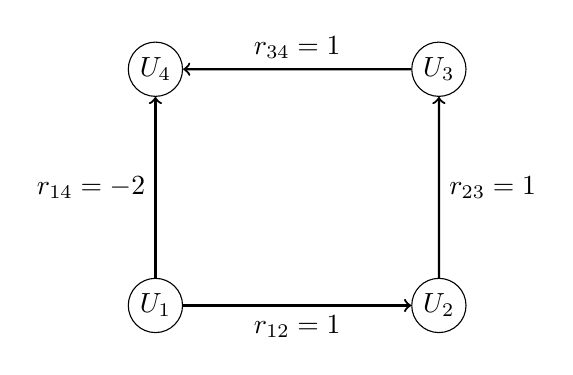
\begin{tikzpicture}[scale=1.5]
\node[circle,draw,inner sep=2pt] (u1) at (0,0) {$U_1$};
\node[circle,draw,inner sep=2pt] (u2) at (2.4,0) {$U_2$};
\node[circle,draw,inner sep=2pt] (u3) at (2.4,2) {$U_3$};
\node[circle,draw,inner sep=2pt] (u4) at (0,2) {$U_4$};
\draw[->,thick] (u1) -- (u2) node[midway,below] {$r_{12}=1$};
\draw[->,thick] (u2) -- (u3) node[midway,right] {$r_{23}=1$};
\draw[->,thick] (u3) -- (u4) node[midway,above] {$r_{34}=1$};
\draw[->,thick] (u1) -- (u4) node[midway,left] {$r_{14}=-2$};
\end{tikzpicture}
\caption{The four-region seam cycle. Vertices are regions, oriented edges are the pairwise seams, and the residue \(r=(1,1,1,-2)\) assigns a rational coefficient to each seam. The residue is closed, since \(C^2=0\), and Proposition~\ref{prop:nonremovable} shows it is not exact.}
\label{fig:fourcycle}
\end{figure}

With the displayed ordering of vertices and edges, the coboundary matrix is
\[
\delta^0=
\begin{pmatrix}
-1&1&0&0\\
0&-1&1&0\\
0&0&-1&1\\
-1&0&0&1
\end{pmatrix},
\]
and \(\delta^1=0\) since \(C^2=0\). For \(b=(b_1,b_2,b_3,b_4)\), this says
\[
\delta^0b=(b_2-b_1,\,b_3-b_2,\,b_4-b_3,\,b_4-b_1).
\]

\begin{proposition}[Four-cycle obstruction witness]\label{prop:nonremovable}
The residue
\[
r=(1,1,1,-2)
\]
determines a non-zero class in \(H^1\).
\end{proposition}

\begin{proof}
Since \(C^2=0\), we have \(\delta^1=0\), hence
\[
\delta^1r=0.
\]
It remains to show that \(r\notin \im\delta^0\). Suppose, for contradiction, that \(r=\delta^0b\) for some \(b=(b_1,b_2,b_3,b_4)\). Then
\[
b_2-b_1=1,
\qquad
b_3-b_2=1,
\qquad
b_4-b_3=1,
\]
so
\[
b_4-b_1
=(b_4-b_3)+(b_3-b_2)+(b_2-b_1)
=3.
\]
But the fourth component of \(\delta^0b=r\) requires
\[
b_4-b_1=-2.
\]
This is impossible. Therefore \(r\notin \im\delta^0\). By Theorem~\ref{thm:classifier-soundness},
\[
0\neq [r]\in H^1.
\]
\end{proof}

The same conclusion is certified by a cycle pairing. Let
\[
z=(-1,-1,-1,1)\in C_1.
\]
A direct calculation gives \(\partial z=0\): each vertex receives one incoming and one outgoing contribution of equal weight around the cycle, so all four components of \(\partial z\) cancel. The pairing with the residue is
\[
\langle z,r\rangle
=(-1)(1)+(-1)(1)+(-1)(1)+(1)(-2)
=-5\neq 0.
\]
By Lemma~\ref{lem:cycle-pairing}, \(r\) is not a coboundary.

\begin{corollary}[Two independent certificates]
The non-zero class \([r]\in H^1\) is certified both by the inconsistent linear system \(\delta^0b=r\) and by the non-zero cycle pairing \(\langle z,r\rangle=-5\).
\end{corollary}


\section{Admissible refinement persistence}
\label{sec:admissible-refinement}

The finite obstruction witness is stated on one presentation of a four-region seam cycle. This section records the general persistence principle used by the refinement witnesses. The statement is deliberately algebraic. It does not claim that every refinement of a regional cover preserves every obstruction. It identifies the conditions under which the displayed cycle-pairing certificate survives passage to a refined finite complex.

Let
\[
C^0 \xrightarrow{\delta^0} C^1 \xrightarrow{\delta^1} C^2
\]
and
\[
C'^0 \xrightarrow{\delta'^0} C'^1 \xrightarrow{\delta'^1} C'^2
\]
be finite cochain complexes over \(\Q\). Write \(Z_1(C)=\ker \partial_1\) for the cycle space dual to \(C^1\), so that every \(z\in Z_1(C)\) pairs with every \(r\in C^1\). A refinement of the residue presentation consists of a cochain map
\[
\rho^*:C^1\longrightarrow C'^1
\]
together with a declared refined cycle \(z'\in Z_1(C')\). It is \emph{certificate-admissible for \((r,z)\)} when the following four conditions hold:
\begin{enumerate}[label=(A\arabic*)]
\item \(\delta^1 r=0\), so \(r\) is closed in the original complex;
\item \(\delta'^1\rho^*r=0\), so the transferred residue is closed in the refined complex;
\item \(z'\) is a cycle in the refined complex, so it annihilates every refined coboundary;
\item \(\langle z',\rho^*r\rangle\neq 0\).
\end{enumerate}
These conditions are weaker than a full comparison theorem between presentations. They are exactly the data required to transport the non-removability certificate.

\begin{theorem}[Cycle-pairing persistence]
\label{thm:witness-persistence}
Let \(r\in C^1\) be a closed residue and let \(\rho^*:C^1\to C'^1\) be a refinement map. If there exists a refined cycle \(z'\in Z_1(C')\) such that
\[
\langle z',\rho^*r\rangle\neq 0,
\]
then \(\rho^*r\notin \im\delta'^0\). Hence \([\rho^*r]\neq 0\in H^1(C')\).
\end{theorem}

\begin{proof}
Assume, for contradiction, that \(\rho^*r=\delta'^0 b'\) for some \(b'\in C'^0\). Since \(z'\) is a cycle, it annihilates refined coboundaries:
\[
\langle z',\delta'^0 b'\rangle=0.
\]
Therefore \(\langle z',\rho^*r\rangle=0\), contradicting the hypothesis. Thus \(\rho^*r\) is not a coboundary. Since it is closed by admissibility, it determines a non-zero class in \(H^1(C')\).
\end{proof}

\begin{theorem}[Universal admissible-refinement persistence]
\label{thm:universal-persistence}
For any finite refinement satisfying conditions \emph{(A1)}--\emph{(A4)} above, the obstruction class of the transferred residue persists in the refined complex.
\end{theorem}

\begin{proof}
Condition \emph{(A2)} gives closedness of \(\rho^*r\), and conditions \emph{(A3)}--\emph{(A4)} supply the non-zero refined cycle pairing. The conclusion is exactly Theorem~\ref{thm:witness-persistence}.
\end{proof}

\begin{remark}[What this theorem does not prove]
The theorem proves persistence under a single declared admissible refinement. It does not prove that two arbitrary presentations determine the same obstruction, nor that every refinement of the cover is admissible. A full presentation-invariance theorem would require comparison of two presentations through a common admissible refinement, with compatibility of the corresponding repair regimes. That stronger problem is outside the scope of this paper.
\end{remark}

\section{Declared presentation changes and refinement witnesses}
\label{sec:invariance-refinement}

This section records the concrete finite witnesses. The general admissible-refinement theorem is proved separately in Section~\ref{sec:admissible-refinement}; the present section shows how the four displayed refinements instantiate it.

\subsection{Presentation invariance}

The following five changes preserve the obstruction verdict: region renaming; edge orientation reversal, with the corresponding sign change; non-zero rational scaling of the residue; gauge perturbation by an exact coboundary; and edge ordering permutation.

\begin{proposition}[Declared presentation invariance]
For the finite object of Section~\ref{sec:actual-witness}, the obstruction verdict
\[
0\neq [r]\in H^1
\]
is invariant under the five declared presentation transformations above.
\end{proposition}

\begin{proof}
Region renaming, edge ordering permutation, and orientation reversal are invertible changes of basis on \(C^0\) and \(C^1\) that commute with the displayed coboundary after transport of structure. Hence they preserve membership in \(\ker\delta^1\) and \(\im\delta^0\), and induce isomorphic cohomology groups. Non-zero scaling multiplies \([r]\) by an element of \(\Q^\times\), so it cannot turn a non-zero class into zero. Finally, exact gauge perturbation sends \(r\) to \(r+\delta^0b\), and \([r+\delta^0b]=[r]\), so the cohomology class does not change at all. Therefore the obstruction verdict is preserved in each case.
\end{proof}

\subsection{Refinement witnesses}

The four refinement witnesses from the original abstract are now re-presented as instances of the admissible-refinement theorem. For each, the four admissibility conditions have been computationally verified. The non-zero pairings are direct consequences of Theorem~\ref{thm:witness-persistence}.

\begin{center}
\begin{tabular}{lll}
\toprule
Refinement Witness & Admissibility & Refined Pairing \(\langle z', \rho^*r \rangle\) \\
\midrule
Subdivide \(U_1\) & Verified & \(-7/2\) \\
Subdivide \(U_2\) & Verified & \(-4\) \\
Subdivide all regions & Verified & \(-5/4\) \\
Insert bridge between \(U_1\) and \(U_2\) & Verified & \(-5\) \\
\bottomrule
\end{tabular}
\end{center}

Each row is a self-contained obstruction certificate: a refined cycle exists and pairs non-trivially with the transferred residue. Therefore each transferred residue is not a coboundary.

\begin{proposition}[Declared Refinement Witnesses as Instances of the Theorem]
Each of the four declared refinements is admissible. By Theorem~\ref{thm:universal-persistence}, the obstruction \([r]\) persists in the refined complex.
\end{proposition}
\begin{proof}
For each of the four witnesses, a refinement morphism \(\rho\) was constructed and all four admissibility conditions were verified computationally using an exact rational solver. The table records the non-zero pairing \(\langle z', \rho^*r \rangle\), which by Theorem~\ref{thm:witness-persistence} certifies that \([\rho^*r] \neq 0\) in the respective refined \(H^1\) group.
\end{proof}

\begin{remark}[Presentation Invariance]
This paper establishes persistence of obstructions under any single admissible refinement. A stronger presentation-invariance theory would compare two different presentations through a common admissible refinement. That problem is not addressed here but is the subject of future work.
\end{remark}

\section{Computational artefact and reproducibility}
\label{sec:repro}

The finite witness of Sections~\ref{sec:certificates} and~\ref{sec:actual-witness} is implemented as an exact rational classifier. The implementation has five roles.

\begin{enumerate}[label=(\arabic*)]
\item It builds the finite coboundary matrices \(\delta^0\) and \(\delta^1\).
\item It checks whether the residue is a cocycle.
\item It solves the linear system \(\delta^0b=r\) over \(\Q\).
\item It emits a certificate containing the cohomology summary and cycle witness.
\item It reruns presentation, refinement, and property-based regression tests.
\end{enumerate}

The witness of Section~\ref{sec:actual-witness} is reproduced by running
\begin{verbatim}
python residue_classifier.py examples/four_cycle.json
\end{verbatim}
against the repository accompanying this paper, with expected verdict
\begin{verbatim}
nontrivial_H1_obstruction
\end{verbatim}
The input file declares the vertices, oriented edges, and residue vector of Figure~\ref{fig:fourcycle}. The emitted certificate is a JSON record with fields for the complex dimensions, the cocycle check \(\delta^1 r=0\), the solver status of \(\delta^0 b=r\), the cycle witness \(z\), and the rational pairing \(\langle z,r\rangle\). The certificates for the refinement witnesses of Section~\ref{sec:invariance-refinement} are stored alongside the example inputs and record the pairings displayed in the table.

The division of labour between proof and computation is as follows. The obstruction verdict for the displayed residue is proved by hand twice, by the linear contradiction and by the cycle pairing of Section~\ref{sec:actual-witness}. The declared presentation-change invariance and admissible-refinement persistence propositions are likewise proved in the text. The code is exactly checked over \(\Q\) with no floating point, and it is regression tested rather than formally verified: a property-based test runs \(1000\) random rational residues on the four-cycle and checks the classifier against the cycle-pairing criterion. On this complex, \(\langle z,r\rangle=0\) exactly when \(r\) is removable, and \(\langle z,r\rangle\neq 0\) exactly when \(r\) represents a nontrivial \(H^1\) obstruction. The current repository state records \(1000\) passed cases and zero failed cases. The computational artefact is therefore not a substitute for the proof. It provides reproducibility, regression protection, and a way of generating further finite witnesses.

\paragraph{Availability of code and data.}
The exact rational classifier, witness files, refinement certificates, and regression tests are available in the repository accompanying this paper. The repository URL will be supplied in the final non-anonymised version. The manuscript's finite obstruction witness can be reproduced by the command displayed above. No empirical data are required.

\section{Scope of results and future work}
\label{sec:scope-future}

The limitations are part of the construction. They mark where the current finite theory is exact, where classification requires extra structure, and where the next mathematical problems begin.

\subsection{Scope of results}

First, the support-refinement axiom is strong. It isolates seam-supported multiplication rather than arbitrary regional multiplication. This makes Theorem~\ref{thm:triple-localisation} clean, but narrows the class of examples.

Second, the first-order variation formula requires a genuine first-order boundary regime. Correction and gauge maps must not reintroduce higher-order dependence on already-boundary terms. This is a guardrail, not a flaw: it is what makes the variation operator linear enough to be written as the four-term expression of Proposition~\ref{prop:four-term}, and it is why Section~\ref{sec:first-order} is a linearised repair calculus rather than a universal repair theorem. Theorem~\ref{thm:square-zero-regime} shows that the regime is not an isolated assumption, since every square-zero regional extension satisfies it by construction, but the restriction to first order remains: outside such regimes the repair problem acquires quadratic terms and takes the shape of a deformation equation rather than a linear system, and the present paper makes no claims there.

Third, the repair quotient \(\Field^2/\im D\) depends on the chosen class of admissible boundary gauges. Different repair regimes may produce different obstruction notions. This dependence is unavoidable, because repair is not a purely formal declaration; it is constrained by which pairwise boundary changes are allowed.

Fourth, \v{C}ech cohomology is not automatic. It requires a coefficient system with restriction maps, an alternating realisation, and a fourfold coherence condition. The paper deliberately keeps these structures separate from the associator field itself, since otherwise one would confuse the finite defect with one possible classification of that defect.

Fifth, the finite residue classifier proves a degree-one obstruction for a declared finite object. It does not by itself classify every associator field, nor does it prove that every triple-seam associator field reduces to a degree-one residue. The two constructions are related by the repair problem of Section~\ref{sec:certificates}, but they are not identical.

Sixth, the refinement persistence result of Section~\ref{sec:admissible-refinement} now rests on a universal theorem, but is demonstrated on only four witnesses. The theorem holds for any refinement satisfying the four admissibility conditions. We do not claim persistence under arbitrary refinements that fail these conditions.

\subsection{Future work}

Four problems are opened by the present construction. The first is realisability: the theory should identify which finite triple-indexed fields can be produced by some supported regional algebra and some admissible boundary correction, separating accidental examples such as Example~\ref{ex:tetrahedron} from structurally forced patterns. The second is an operator-valued theory: the associator field is input-dependent, and a more invariant version would treat associators as operator-valued fields, replacing a static residue with a transformation-level diagnostic that tracks how a seam defect acts on families of inputs. The third is dynamic repair: the present paper treats the regional cover as fixed, whereas in applications the cover may change over time, so a dynamic version would track associator fields over changing nerves and changing admissible repair operators. The fourth is formal verification of the classifier: the executable classifier can be moved from tested Python to a verified kernel in a proof assistant such as Rocq \cite{Rocq2025}. The executable artefact computes certificates, and the proof assistant would certify the classifier's soundness.

\section{Conclusion}

The paper has isolated a finite coherence problem. Pairwise boundary data need not determine coherent ternary gluing. A finite regional system may be locally associative on every region and explicitly corrected on every pairwise seam while still producing a parenthesisation residue on a triple seam. The associator field records that residue before it is forced into any particular classification scheme.

The main structural result is the localisation theorem: under support-refining boundary corrections, the associator defect of a corrected triple product is supported on the common triple overlap. The paper then separates detection, repair, and obstruction. Cohomology enters as a structured classification of the field, not as an assumption built into the field itself. Finally, the paper gives an exact finite obstruction witness: the residue \(r=(1,1,1,-2)\) on a four-region seam cycle is a cocycle but not a coboundary, certified by an explicit contradiction and by the cycle pairing \(\langle z,r\rangle=-5\), invariant under the declared presentation changes, and persistent under the declared admissible refinements.

The resulting claim is modest but sharp. A defect is not an obstruction merely because it is non-zero. It becomes an obstruction only relative to the declared finite compositional apparatus and its admissible repair directions. That is the point at which an associator residue becomes a non-removable coherence failure.

\section*{Declarations}

\paragraph{Funding.}
No funding was received to assist with the preparation of this manuscript.

\paragraph{Competing interests.}
The author declares no competing financial or non-financial interests relevant to the content of this article.

\paragraph{Data availability.}
No empirical datasets were generated or analysed. The finite examples, certificate files, and exact rational checker supporting the manuscript are described in Section~\ref{sec:repro} and will be made available in the repository accompanying the final version.

\paragraph{Code availability.}
The exact rational classifier and accompanying witness files will be made available in the repository accompanying the final version.

\paragraph{Use of AI-assisted tools.}
AI-assisted tools were used during drafting and copy-editing under human direction. The author remains responsible for the final content, mathematical claims, proofs, and presentation.

\appendix

\section{Spectral decomposition of associator fields}
\label{app:spectral}

Cohomology classifies closed defect fields up to coboundary. Before closure is known, one may still analyse a scalar-valued defect field spectrally. This appendix records a finite-dimensional diagnostic layer that is independent of the main results; it uses classical finite Hodge theory on the nerve \cite{Eckmann1944}.

Assume that the nerve \(N(\mathcal U)\) is oriented and that the realised associator field has scalar values in \(\R\), or more generally values in finite-dimensional real inner-product spaces with an induced inner product on cochains. Then the simplicial cochain spaces \(C^n(N;\R)\) carry coboundary maps \(d_n:C^n\to C^{n+1}\) and adjoints \(d_n^*:C^{n+1}\to C^n\) with respect to the standard inner product
\[
\langle \phi,\psi\rangle=\sum_J \phi_J\psi_J,
\]
summed over the oriented \(n\)-simplices \(J\) of the nerve. The degree-two Hodge Laplacian is
\[
\Delta_2=d_1d_1^*+d_2^*d_2.
\]

\begin{theorem}[Spectral decomposition of the associator field]
Assume the nerve \(N(\mathcal U)\) is oriented and that the realised associator field is scalar,
\[
\mathcal A\in C^2(N;\R).
\]
Then \(\mathcal A\) admits a unique orthogonal decomposition
\[
\mathcal A=d_1\theta+H+d_2^*\eta,
\]
where \(d_1\theta\in \im(d_1)\) is the exact component, \(H\in \ker(\Delta_2)\) is the harmonic component, and \(d_2^*\eta\in \im(d_2^*)\) is the coexact component. If, in addition, the scalar realisation identifies admissible pairwise repair with \(d_1\), then the exact component is repairable by pairwise gauge change. If fourfold coherence is tested by \(d_2\), then a non-zero coexact component records failure of fourfold coherence. The harmonic component is the part left by both tests.
\end{theorem}

\begin{proof}
Because \(C^2(N;\R)\) is a finite-dimensional inner-product space, finite Hodge theory yields the orthogonal direct sum
\[
C^2=\im(d_1)\oplus \ker(\Delta_2)\oplus \im(d_2^*).
\]
Projecting \(\mathcal A\) onto the three summands gives the stated decomposition, and orthogonality makes it unique. The identification of these subspaces with operational behaviour is conditional. When the chosen scalar realisation identifies the boundary gauge variation operator \(D\) with \(d_1\), the subspace \(\im(d_1)\) records the repairable directions. When fourfold coherence is tested by \(d_2\), the subspace \(\im(d_2^*)\) records the residual failure of \(d_2\)-closure. The harmonic component is then the part annihilated by both tests.
\end{proof}

\begin{remark}[Fourier language]
The eigenvectors of \(\Delta_2\) play the role of finite Fourier modes on the gluing nerve. Expanding the associator field in these modes reveals whether the defect is concentrated on isolated seams, spread across a global pattern, or carried by harmonic modes. This is a diagnostic use of spectral theory, not a replacement for the algebraic localisation theorem.
\end{remark}

\begin{thebibliography}{99}

\bibitem{Benabou1967}
J. B\'enabou.
\newblock Introduction to bicategories.
\newblock In \emph{Reports of the Midwest Category Seminar}, Lecture Notes in Mathematics 47, pages 1--77. Springer, 1967.

\bibitem{BottTu1982}
R. Bott and L. W. Tu.
\newblock \emph{Differential Forms in Algebraic Topology}.
\newblock Springer, 1982.

\bibitem{CostelloGwilliam2017}
K. Costello and O. Gwilliam.
\newblock \emph{Factorization Algebras in Quantum Field Theory}, Volumes 1 and 2.
\newblock Cambridge University Press, 2017 and 2021.

\bibitem{Curry2014}
J. M. Curry.
\newblock \emph{Sheaves, Cosheaves and Applications}.
\newblock PhD thesis, University of Pennsylvania, 2014.

\bibitem{Eckmann1944}
B. Eckmann.
\newblock Harmonische Funktionen und Randwertaufgaben in einem Komplex.
\newblock \emph{Commentarii Mathematici Helvetici}, 17:240--255, 1944.

\bibitem{EdelsbrunnerHarer2010}
H. Edelsbrunner and J. L. Harer.
\newblock \emph{Computational Topology: An Introduction}.
\newblock American Mathematical Society, 2010.

\bibitem{Ghrist2014}
R. Ghrist.
\newblock \emph{Elementary Applied Topology}.
\newblock Createspace, 2014.

\bibitem{Giraud1971}
J. Giraud.
\newblock \emph{Cohomologie non ab\'elienne}.
\newblock Springer, 1971.

\bibitem{KaczynskiMischaikowMrozek2004}
T. Kaczynski, K. Mischaikow, and M. Mrozek.
\newblock \emph{Computational Homology}.
\newblock Springer, 2004.

\bibitem{KashiwaraSchapira1990}
M. Kashiwara and P. Schapira.
\newblock \emph{Sheaves on Manifolds}.
\newblock Springer, 1990.


\bibitem{Leinster2014}
T. Leinster.
\newblock \emph{Basic Category Theory}.
\newblock Cambridge University Press, 2014.

\bibitem{Riehl2016}
E. Riehl.
\newblock \emph{Category Theory in Context}.
\newblock Dover Publications, 2016.

\bibitem{MacLane1963}
S. Mac Lane.
\newblock Natural associativity and commutativity.
\newblock \emph{Rice University Studies}, 49(4):28--46, 1963.

\bibitem{MacLane1998}
S. Mac Lane.
\newblock \emph{Categories for the Working Mathematician}.
\newblock Second edition. Springer, 1998.

\bibitem{Necula1997}
G. C. Necula.
\newblock Proof-carrying code.
\newblock In \emph{Proceedings of the 24th ACM SIGPLAN-SIGACT Symposium on Principles of Programming Languages}, pages 106--119, 1997.

\bibitem{Robinson2014}
M. Robinson.
\newblock \emph{Topological Signal Processing}.
\newblock Springer, 2014.

\bibitem{Rocq2025}
The Rocq Development Team.
\newblock \emph{The Rocq Prover Reference Manual}.
\newblock 2025. \url{https://rocq-prover.org}.

\bibitem{Vistoli2005}
A. Vistoli.
\newblock Grothendieck topologies, fibered categories and descent theory.
\newblock In \emph{Fundamental Algebraic Geometry: Grothendieck's FGA Explained}, Mathematical Surveys and Monographs 123, pages 1--104. American Mathematical Society, 2005.

\bibitem{Weibel1994}
C. A. Weibel.
\newblock \emph{An Introduction to Homological Algebra}.
\newblock Cambridge University Press, 1994.

\bibitem{Zomorodian2005}
A. Zomorodian.
\newblock \emph{Topology for Computing}.
\newblock Cambridge University Press, 2005.

\end{thebibliography}

\end{document}

